\section{Thema der Abschlussarbeit}
Thema der Abschlussarbeit soll die Umseztung und Gestaltung einer Webanwendung auf Basis von bereits im Praxisprojekt erarbeiteten Konzepten sein.
Die Anwendung hat das Ziel, ihren Nutzern dabei zu helfen, in ihren Gestaltungen eine Grundqualität zu sichern. Die Konzepte wurden speziell auf Studenten des Studiengangs Medieninformatik an der TH Köln ausgelegt. Diese sollen auch die Zielgruppe der Anwendung sein. \\
Ziel der Abschlussarbeit soll es sein, ein funktionierendes und qualitativ hochwertiges Produkt zu erstellen.
Dabei stellen sowohl der Weg vom Konzept und Proof of Concept zum fertigen Produkt als Ablauf, als auch die technische und gestalterische Umsetzung und die damit verbundenen Entscheidungen in den verschiedenen Bereichen die Themengebiete dar, die in der Abschlussarbeit behandelt werden sollen.

Im Praxiprojekt wurde versucht, in verschiedenen Bereichen der visuellen Gerstaltung Regeln und Richtlinien zu definieren, die später von einen Computerprogramm bewertet werden können. Dieser Versuch war in verschiedenen Bereichen wechselndem Erolg. Um die Konzeptarbeit in der Abschlussarbeit möglichst gering zu halten, soll sich in dieser Hauptsächlich auf die bereits gut abgedeckten Bereiche konzentriert werden. Eine Auflistung dieser Bereiche findet sich in \autoref{chapter:setting}: \textit{\nameref{chapter:setting}}.
Weiterhin wurde im Bereich Typografie ein Proof of Concept erstellt, auf dem aufgebaut werden kann.

Im Folgenden sollen die sich für die Abschlussarbeit ergebenden Themengebiete kurz erläutert werden.

\subsection{Genereller Aufbau der Anwendung}
\label{chapter:setting}
Im Rahmen des Praxisprojektes wurden bereits grundlegende Konzepte zu Inhalten der Anwendung in verschiedenen Bereichen erstellt. Da hier nicht in allen Bereichen zufriedenstellende Inhlate gefunden werden konnten, sollen diese als erster Schritt der Abschlussarbeit auf ihre Umsetzbarkeit überprüft werden. Weiterhin muss festgestellt werden, welche Gebiete gegbenenfalls noch weiter vertieft werden müssen.

Die wichtigsten Beispiele für noch nicht hinreichend definierte Bereiche stellen hier der Einstiegspunkt und die Ergebnispräsentation der Anwendung dar.\\
Viele der Kernbereiche der Anwendung greifen auf die verschiedenen Limitationen zurück, die mit den Gestaltungszielen des Nuzters (Plattform, Medium etc.) einher gehen. Diese müssen im ersten Schritt vom Nutzer festgelegt werden. Hier muss bestimmt werden, welche Informationen genau benötigt werden und wie der Nutzer diese der Anwendung mitteilen soll.\\
Auch muss definiert werden, in welcher Form die Anwendung dem Nutzer Ergebnisse mitteilt. So werden dem Nuzter bereits währen der Nutzung implizit Informationen durch seine Interaktion mit der Anwendung mitgeteilt, jedoch besteht bisher kein Konzept, nach dem diese dem Nutzer am Ende der Anwendung noch einmal geordnet zur Weiterverwendung angeboten werden.

In einer ersten funktionierenden Version der Anwednung sollten die folgenden Bereiche enthalten sein:

\begin{itemize}
  \item Einstieg
  \item Typographie
  \item Layout \& Grid
  \item Farben
  \item Ergebnisse
\end{itemize}

Je nach Zeitlichem verlauf können diese noch um weitere Themengebiete erweitert werden.

\subsection{Technologien und Architektur}
Auch die Architektur der Anwendung und die zu verwendenden Technologien sollen im Rahmen der Abschlussarbeit diskutiert werden.

Die Anwendung soll mit Hilfe des Framework React.js umgesetzt werden. React.js ist ein Javascript-Framework, das 2013 von Facebook entwickelt wurde. \cite{gackenheimer2015react} beschreibt React wie folgt:

\begin{quote}
[...] React is a way to describe the user interface of an application and a mechanism to change that over time as data changes. React is made with declarative components that describe an interface. React uses no observable data binding when building an application. React is also easy to manipulate, because you can take the components you create and combine them to make custom components that work as you expect every time because it can scale.
\end{quote}

Der Fokus des Framworks liegt also auf interaktiven User Interfaces, in denen sich die enthaltenen Daten häufig ändern. Da die Anwenundung dem Nuzter ineraktives Feedback zu seinen Eingaben geben soll, ist React.js hier gut geeigent. Der Proof of Concept im Praxisprojekt wurde bereits erfolgreich mit Hilfe von React.js umgesetzt und unterstützt die Entscheidung zur Wahl des Frameworks weiter. \\

Da für die Anwendung keine persistente Datenhaltung benötigt wird, kann auf eine klassische Client-Server-Architektur verzichtet werden und die komplette Logik kann auf dem Client ausgeführt werden.\\
Trotzdem sollte auch im Client eine Architektur entworfen werden. Wie oben bereits erwähnt stehen Teile der Anwendung in Abhängigkeit zueinander und Daten aus frühren Schritte beeinflussen die Darstellung von späteren\footnotemark[1]. Deshalb soll zu beginn ein Modell der Anwendung und der Datenhaltung angefertigt werden. Für die Datenhaltung soll dabei auf redux zurückgegriffen werden.

\subsubsection{Redux}
Redux verwaltet den Zustand (oder \textit{state}) einer Anwendung und sorgt dafür, dass dieser Konsistent bleibt. Diese Konsistenz wird durch drei Grunprinzipien von redux erreicht \cite{threeprinciplesredux}:

\begin{enumerate}
  \item Der Zustand wir nur an einer zentralen Stelle verwaltet.
  \item Der Zustand kann nur gelesen und nicht direkt manipuliert werden.
  \item Der Zustand kann nur durch \textit{pure functions}\footnotemark[2] verändert werden.
\end{enumerate}

Redux wurde bereits beim Proof of Concept für den Bereich Typographie im Praxisprojekt verwendet. Hier konnte der Nutzer Werte von verschiedenen typografischen Elementen (z.B. Schriftgröße oder Zeilenhöhe) ändern, die dann verschiedene DOM-Elemente beeinflussten (beispielsweise ein \textit{range input} und eine Darstellung des generieten Textes). Mit Hilfe von Redux konnte dafür gesorgt werden, dass trotz der verschiedenen Komponenten, die auf einen Wert angewiesen waren, dieser im \textit{state} nicht überschrieben wurde.

\subsection{Gestaltung der Anwendung}
Auch die Gestaltung der Anwendung soll Teil der Bachelorarbeit sein. Hier soll darauf geachtet werden, dass die Anwendung möglichst neutral gestaltet wird, um den Fokus des Nutzers nicht von seiner eigenen Gestaltungsarbeit abzulenken.\\
Der Designprozess soll auf das komponentenbasierte Verhalten von React.js angepasst sein. Ganze Seiten sollen  nur in Form von Wireframes erstellt werden, in denen auch Inhalte und Interaktionen festgelegt werden sollen. Einzelne Komponenten auf den Seiten sollen im Detail gestaltet werden, sodass am Ende des Designporzesses ein Verzeichnis von Komponenten entsteht, die in der Anwendung verwendet werden können.

Um dieses Verzeichnis auch in die Anwendung übernehmen zu können, soll auf \textit{Stroybook for React} zurück gegriffen werden \cite{StorybooksOnline}, das es ermöglicht, einen \textit{living styleguide} für die Verwendung in der Anwendung zu erstellen. Der Code für die verschiedenen Komponenten im Stroybook ist dabei der gleiche, der auch in der Anwendung verwendet wird. Im Stroybook können außerdem verschiedene Stati und auch Funktionen der Komponenten abgebildet werden. \textit{Abbildung \ref{fig:storybook}} auf Seite \pageref{fig:storybook} zeigt dies am Beispiel von einem Button.

\begin{figure}[h]
  \centering
  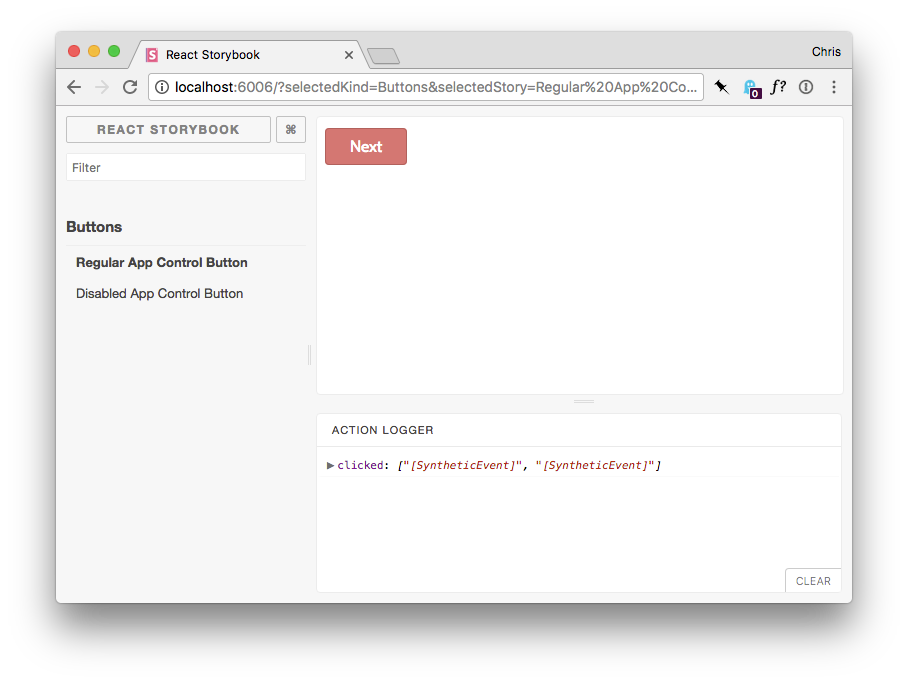
\includegraphics[width=1\textwidth]{images/ReactStroybooksExample.png}
  \caption{Beispielhafte Verwendung von \textit{Stroybook for React} mit einem Button}
  \label{fig:storybook}
\end{figure}

Durch die komponentenbasierte Form von React bietet es sich an, auch CSS direkt in eine Komponente zu schreiben. So sind Komponenten sowohl in ihrer Funktion, als auch in ihrem Aussehen in sich abgeschlossene und weitestgehend unabhängige Teile der Anwendung. Auch dieses vorgehen soll in der Abschlussarbeit weiter thematisiert werden.

\section{Relevanz des Themas}
Die Relevanz der Anwendung an sich wurde bereits im Praxisprojekt erläutert, daher soll hier nur eine Kurzfassung der Erläuterung folgen:\\
Lindgaard et al. \cite{lindgaard2006attention} haben gezeigt, dass Menschen sich in nur 50ms ein Urteil über die Gestaltung einer Website bilden. Der erste Eindruck spielt bei Menschen auch bei der späteren Bewertung einer Sache noch eine wichtige Rolle \cite{campbell1996fitting}. Von diesem ersten Eindruck lassen sich Menschen nur schwer wieder abbringen \cite{nickerson1998confirmation}.
Daher ist es wichtig, dass auch Artefakte in Modulen, in denen die Gestaltung gegebenenfalls nicht bewertet wird, ein solides Design aufweisen, um den ersten Eindruck so positiv wie möglich zu gestalten.

Unterstützend seien hier noch zwei weitere Quellen aufgeführt, die die Relevanz weiter unterstreichen:\\
\cite{tractinsky2006evaluating} zeigen, dass die Ergebnisse der Studie von Lingaard et al. auch mit anderen Parametern bestand haben und unterstreichen weiterhin die Wichtigkeit von guter Gestaltung für eine gute Nutzerefahrung \cite{tractinsky2000beautiful}.\\
Auch aus vielen persönlichen Gespräche konnte ich entnehmen, dass die Umsetzung der erarbeiteten Konzepte als Produkt, auch für verschiedene Personengruppen, durchaus wünschenswert ist.

Neben der Relevanz des Produktes, das in Rahmen der Arbeit entstehen soll ist aber auch das eigentliche Thema der Arbeit zu rechtfertigen: Die Entwicklung von einem Konzept zu einem fertigen Produkt.
Als abschließende Arbeit für den Studiengang Medieninformatik ist dies ein passendes Thema, da in diesem viele Aspekte das gesamten Studiums vereint werden. In den weiter oben genannten Bereichen kommen besiepielsweis Inhalte aus den Modulen GdvK, WBA 1, ST,  PM und EIS vor. Daher bietet das Thema eine gute Verbindung zwischen den verschiedenen Disziplinen innerhalb des Studiums, verbunden mit einer wissenschaftlichen Disukssion verschiedener Vorgehensweisen und Abläufe.

\section{Organisatorisches}

Im folgenden seien auch einige organisatorische Aspekte im Bezug auf die Druchführung der Arbeit angesprochen. Anbei finden sich eine erste, grobe Gliederung der Arbeit und ein erster Zeitplan.

\subsection{Erste Gliederung}
Es sei angemerkt, dass die folgende Gleiderung keinen Anspruch auf Vollständigkeit besitzt und auch während der Druchführung der Arbeit bei bedarf noch verändert werden kann.
Gerade für den zweiten Teil gestaltet es sich schwierig, genauere Voraussagen über den Inhalt zu machen, da viele der Artefakte, durch die dieser Teil definiert wird, noch nicht existieren.

\begin{itemize}
  \item Einleitung
  \item Relevanz des Themas
  \item Zielsetzung der Arbeit
  \item 1.Teil: Theoretische Grundlagen
  \begin{enumerate}
    \item Struktur der Anwendung
    \begin{enumerate}
      \item Stand Praxisprojekt
      \item Einstieg
      \item Ergebnisse
    \end{enumerate}
    \item Verwendete Technologie
    \begin{enumerate}
      \item React.js
      \item redux
      \item Storybooks for React
    \end{enumerate}
    \item Vorgehen bei der Gestaltung
  \end{enumerate}
  \item 2.Teil: Umsetzung
  \begin{enumerate}
    \item Gestaltung
    \begin{enumerate}
      \item Wireframes
      \item High-Fidelity-Komponenten
    \end{enumerate}
    \item Aufbau der Anwendung
    \begin{enumerate}
      \item Redux
      \item CSS-Architektur
      \item React Storybooks
    \end{enumerate}
    \item Beispielhafte Algorithmen
  \end{enumerate}
  \item Fazit
  \item Ausblick
\end{itemize}

\subsection{Zeitplan und Organisation}
Die Arbeit soll so bald wie möglich, spätestens aber am 31.5.2017 angemeldet werden. Da kein erhöhter empirischer Anteil besteht, ist die reguläre Dauer von 9 Wochen zur Beendigung der Arbeit vorgesehen. Die Arbeit soll also (je nach Anmeldung) spätestens in der ersten Augustwoche 2017 abgegeben werden.

Als zweitprüferin ist Dipl. Des. Liane Kirschner vorgesehen, die aktuell bei der Railslove GmbH in Köln tätig ist.


\footnotetext[1] {Als Beispiel wäre hier der Bereich Farben zu nennen, wenn der Nutzer für das mobile Betriebssystem Android gestaltet. Hier werden dann nur die in den Material Design Guidelines definierten Farben als Auswahl angeboten.}
\footnotetext[2] {\textit{pure functions} sind funktionen, die keine Nebeneffekte aufweisen, also beim Aufruf mit den gleichen Argumenten zwangsweise die gleichen Ergebnisse liefern \cite{Haverbeke201412}. So kann eine Funktion, deren Ergbnis beispielsweise vom aktuellen Datum abhängt, niemlas \textit{pure} sein.}
